\documentclass{article}
\usepackage{graphix}
\usepackage[title]{appendix}
% if you need to pass options to natbib, use, e.g.:
%     \PassOptionsToPackage{numbers, compress}{natbib}
% before loading neurips_2024


% ready for submission
% \usepackage{neurips_2024}


% to compile a preprint version, e.g., for submission to arXiv, add add the
% [preprint] option:
%  \usepackage[preprint]{neurips_2024}


% to compile a camera-ready version, add the [final] option, e.g.:
\usepackage[final]{neurips_2024}


% to avoid loading the natbib package, add option nonatbib:
%    \usepackage[nonatbib]{neurips_2024}


\usepackage[utf8]{inputenc} % allow utf-8 input
\usepackage[T1]{fontenc}    % use 8-bit T1 fonts
\usepackage{hyperref}       % hyperlinks
\usepackage{url}            % simple URL typesetting
\usepackage{booktabs}       % professional-quality tables
\usepackage{amsfonts}       % blackboard math symbols
\usepackage{nicefrac}       % compact symbols for 1/2, etc.
\usepackage{microtype}      % microtypography
\usepackage{xcolor}         % colors

% Redefine the footer command to remove the footer
\makeatletter
\renewcommand{\@noticestring}{}
\makeatother

\title{CMSC 35300 Course Project Report: Gesture Classification and Prediction}


% The \author macro works with any number of authors. There are two commands
% used to separate the names and addresses of multiple authors: \And and \AND.
%
% Using \And between authors leaves it to LaTeX to determine where to break the
% lines. Using \AND forces a line break at that point. So, if LaTeX puts 3 of 4
% authors names on the first line, and the last on the second line, try using
% \AND instead of \And before the third author name.

\author{
  Lan Gao \\
  Department of Computer Science \\
  University of Chicago \\
  \texttt{langao@uchicago.edu} \\
  \And
  Sam Cong \\
  Social Science Division \\
  University of Chicago \\
  \texttt{tianyuec@uchicago.edu} \\
  \And
  Yun Ho \\
  Department of Computer Science \\
  University of Chicago \\
  \texttt{yunho@uchicago.edu} \\
}


\begin{document}


\maketitle


\begin{abstract}
  This project explores how machine learning techniques, including but not limited to k-nearest neighbors (KNN), support vector machines (SVM), and principal component analysis (PCA), could be used to fulfill image processing, prediction, and completion in real practice. Building upon an image dataset of sign language digits photos, we train machine learning models using different algorithms for two tasks: sign language digits prediction and sign language digits completion. Our result shows that in the sign language digits prediction task, SVM performs best in the k-fold validation while KNN performs best in the testing set. Whereas in the sign language digits completion task, we find Kernal Ridge Regression (KRR) outperforms other algorithms. Our project extends the lecture content by examining the usage and performance of different machine-learning algorithms in different image-based tasks.
\end{abstract}


\section{Introduction}
Machine learning has been widely used to understand and process image information in real-world applications. In this project, we aim to explore the performance of fundamental machine learning algorithms, by conducting image processing, prediction, and completion tasks in real-world cases. Our project was conducted on a sign language digit dataset, which contains 2062 photos of sign language classified into 10 categories that represent digits 0-9 respectively. After preprocessing images in the dataset into image feature matrix and ground truth labels of representing digits, we ran the following two experiments: 1) training and testing different machine learning models that predict which digit a sign language stands for given a photo (refers to 'sign language digits prediction' from here on); and 2) extracting the key image features and training a machine learning model that predicts the lower half of sign language digit photo, given the upper half of the photo (refers to 'sign language digits completion' from here on).

In the sign language digits prediction task, we employed three traditional machine learning algorithms—k-nearest neighbors (KNN), random forest, and support vector machines (SVM)—to classify sign language digits based on image data. The process began by utilizing the image feature matrix as the input variable (X) and the corresponding ground truth labels as the target variable (y). To ensure robust model evaluation, we implemented K-fold cross-validation alongside performance assessment on a separate testing dataset. This approach facilitated the comparison of the predictive capabilities of each algorithm under consistent evaluation conditions.

For the sign language digits completion task, we reconstructed the lower half of each image based on the upper half. Specifically, the goal was to predict the missing lower half lever- aging information from the upper half, allowing the model to “complete” the image of each sign language digit. To achieve this, we experimented with various approaches, including ridge regression, principal component regression, and kernel ridge regression. Furthermore, we evaluated and compared model performance using metrics such as mean squared error (MSE), Structural Similarity Index Measure (SSIM), and Peak Signal-to-Noise Ratio (PSNR). Finally, we explained the differences in model performance and suggested potential ways to improve performance.

While deep learning approaches have become the predominant methods in real-world image understanding and processing applications, we hypothesize that traditional machine learning algorithms can still deliver robust performance on image-based tasks. Specifically, we propose that traditional algorithms may offer significant advantages in scenarios where computational resources are limited and where moderate levels of accuracy are acceptable. This suggests that, despite the advancements in deep learning, traditional machine learning techniques remain valuable alternatives for specific applications that prioritize lower computational costs without substantial compromises in performance

\section{Literature Review}
\subsection{Image Prediction: the Case of Sign Language Prediction}
Sign language prediction is a widely researched application of machine learning for image processing. To recognize sign language from images, raw photos of sign language usually undergo image acquisition, image pre-processing, segmentation, feature extraction, and classification (Adeyanju et al., 2021). In our project, we mainly focus on the classification tasks.

Computer vision methods through deep learning, such as Convolutional Neural Networks (CNN), are the state-of-the-art approaches adopted by most researchers to process sign language classification (Aggarwal et al., 2023). However, traditional machine learning algorithms are also been used for fundamental classifiers, especially for those tasks targeting minority sign languages. For example, Tharwat et al. developed an Arabic sign language recognition system, which was based on Scale Invariant Features Transform
(SIFT) for feature extraction with Linear Discriminant Analysis (LDA) for dimensionality reduction, and SVM and KNN (k=1 and k=5) for classification. Their experiments showed that SVM outperforms KNN in all tasks, including normal prediction, prediction on rotated signs, and prediction on occlusion images (Tharwat et al., 2015).

\subsection{Image Completion}
Image completion is a technique to reconstruct a missing part of an image. Real-world image completion tasks usually only use the visible part of an image as the training dataset, inferring the missing part based on the context provided in the existing part. For example, Drori et al. proposed a fragment-based image completion approach, where they used a fast approximation to iteratively select image fragments that were the most frequent and common in the visible image part. As the selected segments are synthesized, their likelihood increases along with the mean confidence of the image, by which a final image was synthesized (Drori et al., 2003). The context of image completion is a key factor that influences the performance. Regarding that, Iizuka et al. built an image completion system with fully-CNNs to predict and fill the missing part, which was trained with global and local context discriminator networks recognizing whole image consistency and small area consistency, respectively. Their experiment shows an outperformance of most state-of-the-art image completion approaches (Iizuka et al., 2017). 

Our project, unlike prior works that only use limited training data and advanced deep learning approaches, investigates how traditional machine learning algorithms work on image completion with enough training data of similar complete images.

\section{Dataset}
In this project, we conducted our experiments in the Sign Language Digits Dataset,\footnote{https://github.com/ardamavi/Sign-Language-Digits-Dataset} an open dataset of a collection of sign language digit images. This dataset was designed for recognizing hand signs corresponding to digits 0-9 in American Sign Language. 

The raw dataset contains 2062 photos of hand signs with each one 100x100 pixels, which were classified into 10 classes representing digits 0-9. Before running experiments, all raw images undergo several preprocessing steps, including image resizing to a fixed dimension (specifically, 64x64 pixels), label assignment via one-hot encoding, and normalization of pixel values to enhance contrast in grayscale data. This processing results in 2062 samples, each of which has a 64x64 image feature matrix, and a corresponding numeric ground truth label, standing for 10 different digit signs from 0-9.


\section{Sign Language Digits Prediction}
We used three traditional machine learning algorithms, k-nearest neighbors (KNN), random forest, and support vector machines (SVM), to predict the sign language digits (0-9) from the hand-pose images. First, we split the dataset (i.e., 2062 images and their ground truth labels) into training and testing datasets. We withheld 20\% of the images as testing data. Then, we trained the classification models with KNN, random forest, and SVM. For KNN, the number of neighbors was set to three, and the average score from 10-fold cross-validation was 0.61 with a standard deviation of 0.03. For random forest, the average score from 10-fold cross-validation was 0.39 with a standard deviation of 0.04. For SVM classification, the average score from 10-fold cross-validation was 0.83 with a standard deviation of 0.03.
Finally, we test the performance (i.e., prediction accuracy) of our prediction models with the testing data. The accuracy of the KNN model was 0.946; the accuracy of the random forest model was 0.94, and the accuracy of the SVM model was 0.847.
TODO: why cross validation SVM best, and why prediction SMV worst (e.g., overfitting)

\section{Sign Language Digits Completion}
We utilized traditional regression-based methods to determine how well they can reconstruct the missing lower half of each image using information from the upper half. Specifically, each image is initially flattened into a 4096-dimensional vector ($64 \times 64$ pixels). The dataset is split into 80\% training and 20\% testing, ensuring the separation occurs before dividing each image into upper and lower halves to prevent data leakage. After splitting, the upper half of the images forms the input features ($X$), while the lower half serves as the target variables ($y$). This setup ensures that our models learn to predict the missing lower part of the image solely from the visible upper part.

We adopted three regression-based models for the image completion task: Ridge Regression (RR), Principal Component Regression (PCR), and Kernel Ridge Regression (KRR). Ridge Regression adds an $L_2$ penalty to reduce overfitting and stabilize predictions (see Appendix \ref{app:ridge_regression}). PCR combines principal component analysis (PCA) for dimensionality reduction with linear regression, retaining the first 50 principal components that capture the majority of variation in the data (see Appendix \ref{app:pcr_regression}). KRR extends Ridge Regression into the nonlinear domain by introducing a kernel function, specifically the Radial Basis Function (RBF) kernel, which allows the model to capture more complex patterns in the data (see Appendix \ref{app:krr_regression}). Hyperparameters for these models are optimized through cross-validation to identify the best combinations of regularization strength and kernel parameters (for KRR).

We evaluated each model’s performance using three metrics: mean squared error (MSE), Structural Similarity Index Measure (SSIM), and Peak Signal-to-Noise Ratio (PSNR; see Appendix \ref{app:evaluation_metrics}). MSE measures the average squared difference between predicted and actual pixel values. SSIM assesses the structural similarity between the reconstructed and original images, capturing perceptual quality better than MSE alone. PSNR provides a logarithmic measure of reconstruction quality in decibels, with higher values indicating better reconstructions. The evaluation process involves reshaping the predicted and actual lower halves to their original dimensions, computing MSE, SSIM, and PSNR on a per-image basis, and then averaging the metrics over all test images. Special care is taken in the case of MSE=0, where PSNR approaches infinity, indicating perfect reconstruction.

The results, presented in Table \ref{table:model_comparison}, show a clear performance hierarchy among the three methods. KRR achieves the best overall performance, featuring the lowest MSE, highest SSIM, and highest PSNR. This suggests that the non-linear flexibility offered by the RBF kernel is particularly advantageous for capturing the complex patterns required to reconstruct missing image portions accurately. PCR provides intermediate performance, indicating that dimensionality reduction preserves sufficient information for moderate-quality reconstructions. RR, by contrast, exhibits the weakest results, highlighting the limitations of purely linear methods in this more complex completion task. A visual comparison of reconstruction quality is provided in Appendix \ref{app:image_comparison}, demonstrating that KRR preserves subtle image details and smooth transitions more effectively than the other methods.

These findings highlight the importance of modeling non-linear patterns for image completion. Although traditional methods do not match the performance of advanced deep learning techniques, KRR’s success suggests that careful kernel design and feature transformation can yield significant improvements. Future work could involve experimenting with alternative kernel functions, incorporating more sophisticated dimensionality reduction techniques, or integrating deep learning approaches like autoencoders and generative adversarial networks (GANs) to potentially achieve even higher quality reconstructions.

\begin{table}[h]
    \centering
    \caption{Performance Comparison of Different Regression Methods}
    \begin{tabular}{l
                    S[table-format=1.4]
                    S[table-format=1.4]
                    S[table-format=2.2]}
    \toprule
    {Method} & {MSE} & {SSIM} & {PSNR} \\
    \midrule
    RR & 0.0153 & 0.4045 & 18.5663 \\
    PCR & 0.0131 & 0.4251 & 19.0970 \\
    KRR & 0.0123 & 0.4425 & 19.4289 \\
    \bottomrule
    \end{tabular}
\label{table:model_comparison}
\end{table}

% Start the "References" section in a new page
\newpage
\section*{References}
\medskip


{
\small


[1] Adeyanju, I. A., Bello, O. O., \& Adegboye, M. A. (2021). Machine learning methods for sign language recognition: A critical review and analysis. Intelligent Systems with Applications, 12, 200056.


[2] Aggarwal, D., Ahirwar, S., Srivastava, S., Verma, S., \& Goel, Y. (2023, March). Sign Language Prediction using Machine Learning Techniques: A Review. In 2023 Second International Conference on Electronics and Renewable Systems (ICEARS) (pp. 1296-1300). IEEE.


[3] Tharwat, A., Gaber, T., Hassanien, A. E., Shahin, M. K., \& Refaat, B. (2015). Sift-based arabic sign language recognition system. In Afro-European Conference for Industrial Advancement: Proceedings of the First International Afro-European Conference for Industrial Advancement AECIA 2014 (pp. 359-370). Springer International Publishing.


[4] Drori, I., Cohen-Or, D., \& Yeshurun, H. (2003). Fragment-based image completion. In ACM SIGGRAPH 2003 Papers (pp. 303-312).


[5] Iizuka, S., Simo-Serra, E., \& Ishikawa, H. (2017). Globally and locally consistent image completion. ACM Transactions on Graphics (ToG), 36(4), 1-14.
}


% %%%%%%%%%%%%%%%%%%%%%%%%%%%%%%%%%%%%%%%%%%%%%%%%%%%%%%%%%%%%
\begin{appendices}
\clearpage
\section*{Appendices}
\addcontentsline{toc}{section}{Appendices}

\section{Ridge Regression Formula} \label{app:ridge_regression}
The Ridge Regression (RR) implementation involved standardizing both input features and target variables, followed by ridge regression with cross-validation. The optimization problem for ridge regression is:

\begin{equation}
    \hat{\beta}_{ridge} = \argmin_{\beta} \left\{ \|y - X\beta\|^2 + \alpha\|\beta\|^2 \right\}
\end{equation}

where:
\begin{itemize}
    \item $X$ is the standardized input matrix
    \item $y$ is the standardized target vector
    \item $\alpha$ is the regularization parameter, tested for values $\{0.1, 1.0, 10.0, 100.0\}$
    \item $\|\beta\|^2$ is the L2 norm of the coefficient vector
\end{itemize}

\section{Principal Component Regression Formula} \label{app:pcr_regression}
PCR combines PCA with linear regression. The PCA transformation is first computed as:

\begin{equation}
    Z = X W
\end{equation}

where:
\begin{itemize}
    \item $W$ is the matrix of eigenvectors of $X^TX$
    \item $Z$ represents the principal components
\end{itemize}

The first 50 components are retained, and linear regression is performed:

\begin{equation}
    y = Z_{50}\gamma + \epsilon
\end{equation}

where:
\begin{itemize}
    \item $Z_{50}$ contains the first 50 principal components
    \item $\gamma$ is the coefficient vector in the transformed space
    \item $\epsilon$ is the error term
\end{itemize}

\section{Kernel Ridge Regression Formula} \label{app:krr_regression}
KRR extends ridge regression to non-linear patterns using the kernel trick. The optimization problem becomes:

\begin{equation}
    \hat{\alpha} = \argmin_{\alpha} \left\{ \|y - K\alpha\|^2 + \lambda\alpha^T K\alpha \right\}
\end{equation}

with the RBF kernel function:

\begin{equation}
    K(x_i, x_j) = \exp\left(-\gamma\|x_i - x_j\|^2\right)
\end{equation}

where:
\begin{itemize}
    \item $K$ is the kernel matrix with elements $K_{ij} = K(x_i, x_j)$
    \item $\gamma$ is the RBF kernel coefficient
    \item $\lambda$ is the regularization parameter
    \item The prediction for a new point $x_*$ is given by:
    \begin{equation}
        f(x_*) = \sum_{i=1}^n \alpha_i K(x_i, x_*)
    \end{equation}
\end{itemize}

Hyperparameters were optimized through 5-fold cross-validation:
\begin{itemize}
    \item Regularization parameter $\lambda \in \{0.001, 0.01, 0.1, 1.0, 10.0\}$
    \item RBF kernel coefficient $\gamma \in \{0.0001, 0.001, 0.01, 0.1, 1.0\}$
\end{itemize}

\section{Evaluation Metrics} \label{app:evaluation_metrics}
Three different metrics were used to evaluate the quality of the image reconstruction:

\paragraph{Mean Squared Error (MSE)}
MSE measures the average squared difference between predicted and actual pixel values:
\begin{equation}
    MSE = \frac{1}{n} \sum_{i=1}^{n} (y_i - \hat{y}_i)^2
\end{equation}
where $y_i$ represents the true pixel values and $\hat{y}_i$ represents the predicted pixel values.

\paragraph{Structural Similarity Index Measure (SSIM)}
SSIM evaluates the perceived quality between two images $x$ and $y$ by combining three comparative measurements:
\begin{equation}
    SSIM(x,y) = \frac{(2\mu_x\mu_y + c_1)(2\sigma_{xy} + c_2)}{(\mu_x^2 + \mu_y^2 + c_1)(\sigma_x^2 + \sigma_y^2 + c_2)}
\end{equation}
where:
\begin{itemize}
    \item $\mu_x$, $\mu_y$ are the average pixel values
    \item $\sigma_x^2$, $\sigma_y^2$ are the variances
    \item $\sigma_{xy}$ is the covariance
    \item $c_1$, $c_2$ are constants to avoid division by zero
\end{itemize}
SSIM ranges from -1 to 1, with 1 indicating perfect structural similarity.

\paragraph{Peak Signal-to-Noise Ratio (PSNR)}
PSNR measures the ratio between the maximum possible pixel value and the corrupting noise:
\begin{equation}
    PSNR = 20 \cdot \log_{10}\left(\frac{MAX_I}{\sqrt{MSE}}\right) = 20 \cdot \log_{10}\left(\frac{1}{\sqrt{MSE}}\right)
\end{equation}
where $MAX_I$ is the maximum possible pixel value (normalized to 1 in our case). PSNR is expressed in decibels (dB), with higher values indicating better quality reconstruction.

\newpage
\section{Image Completion Model Comparison Figure} \label{app:image_comparison}
\begin{figure}[h]
    \centering
    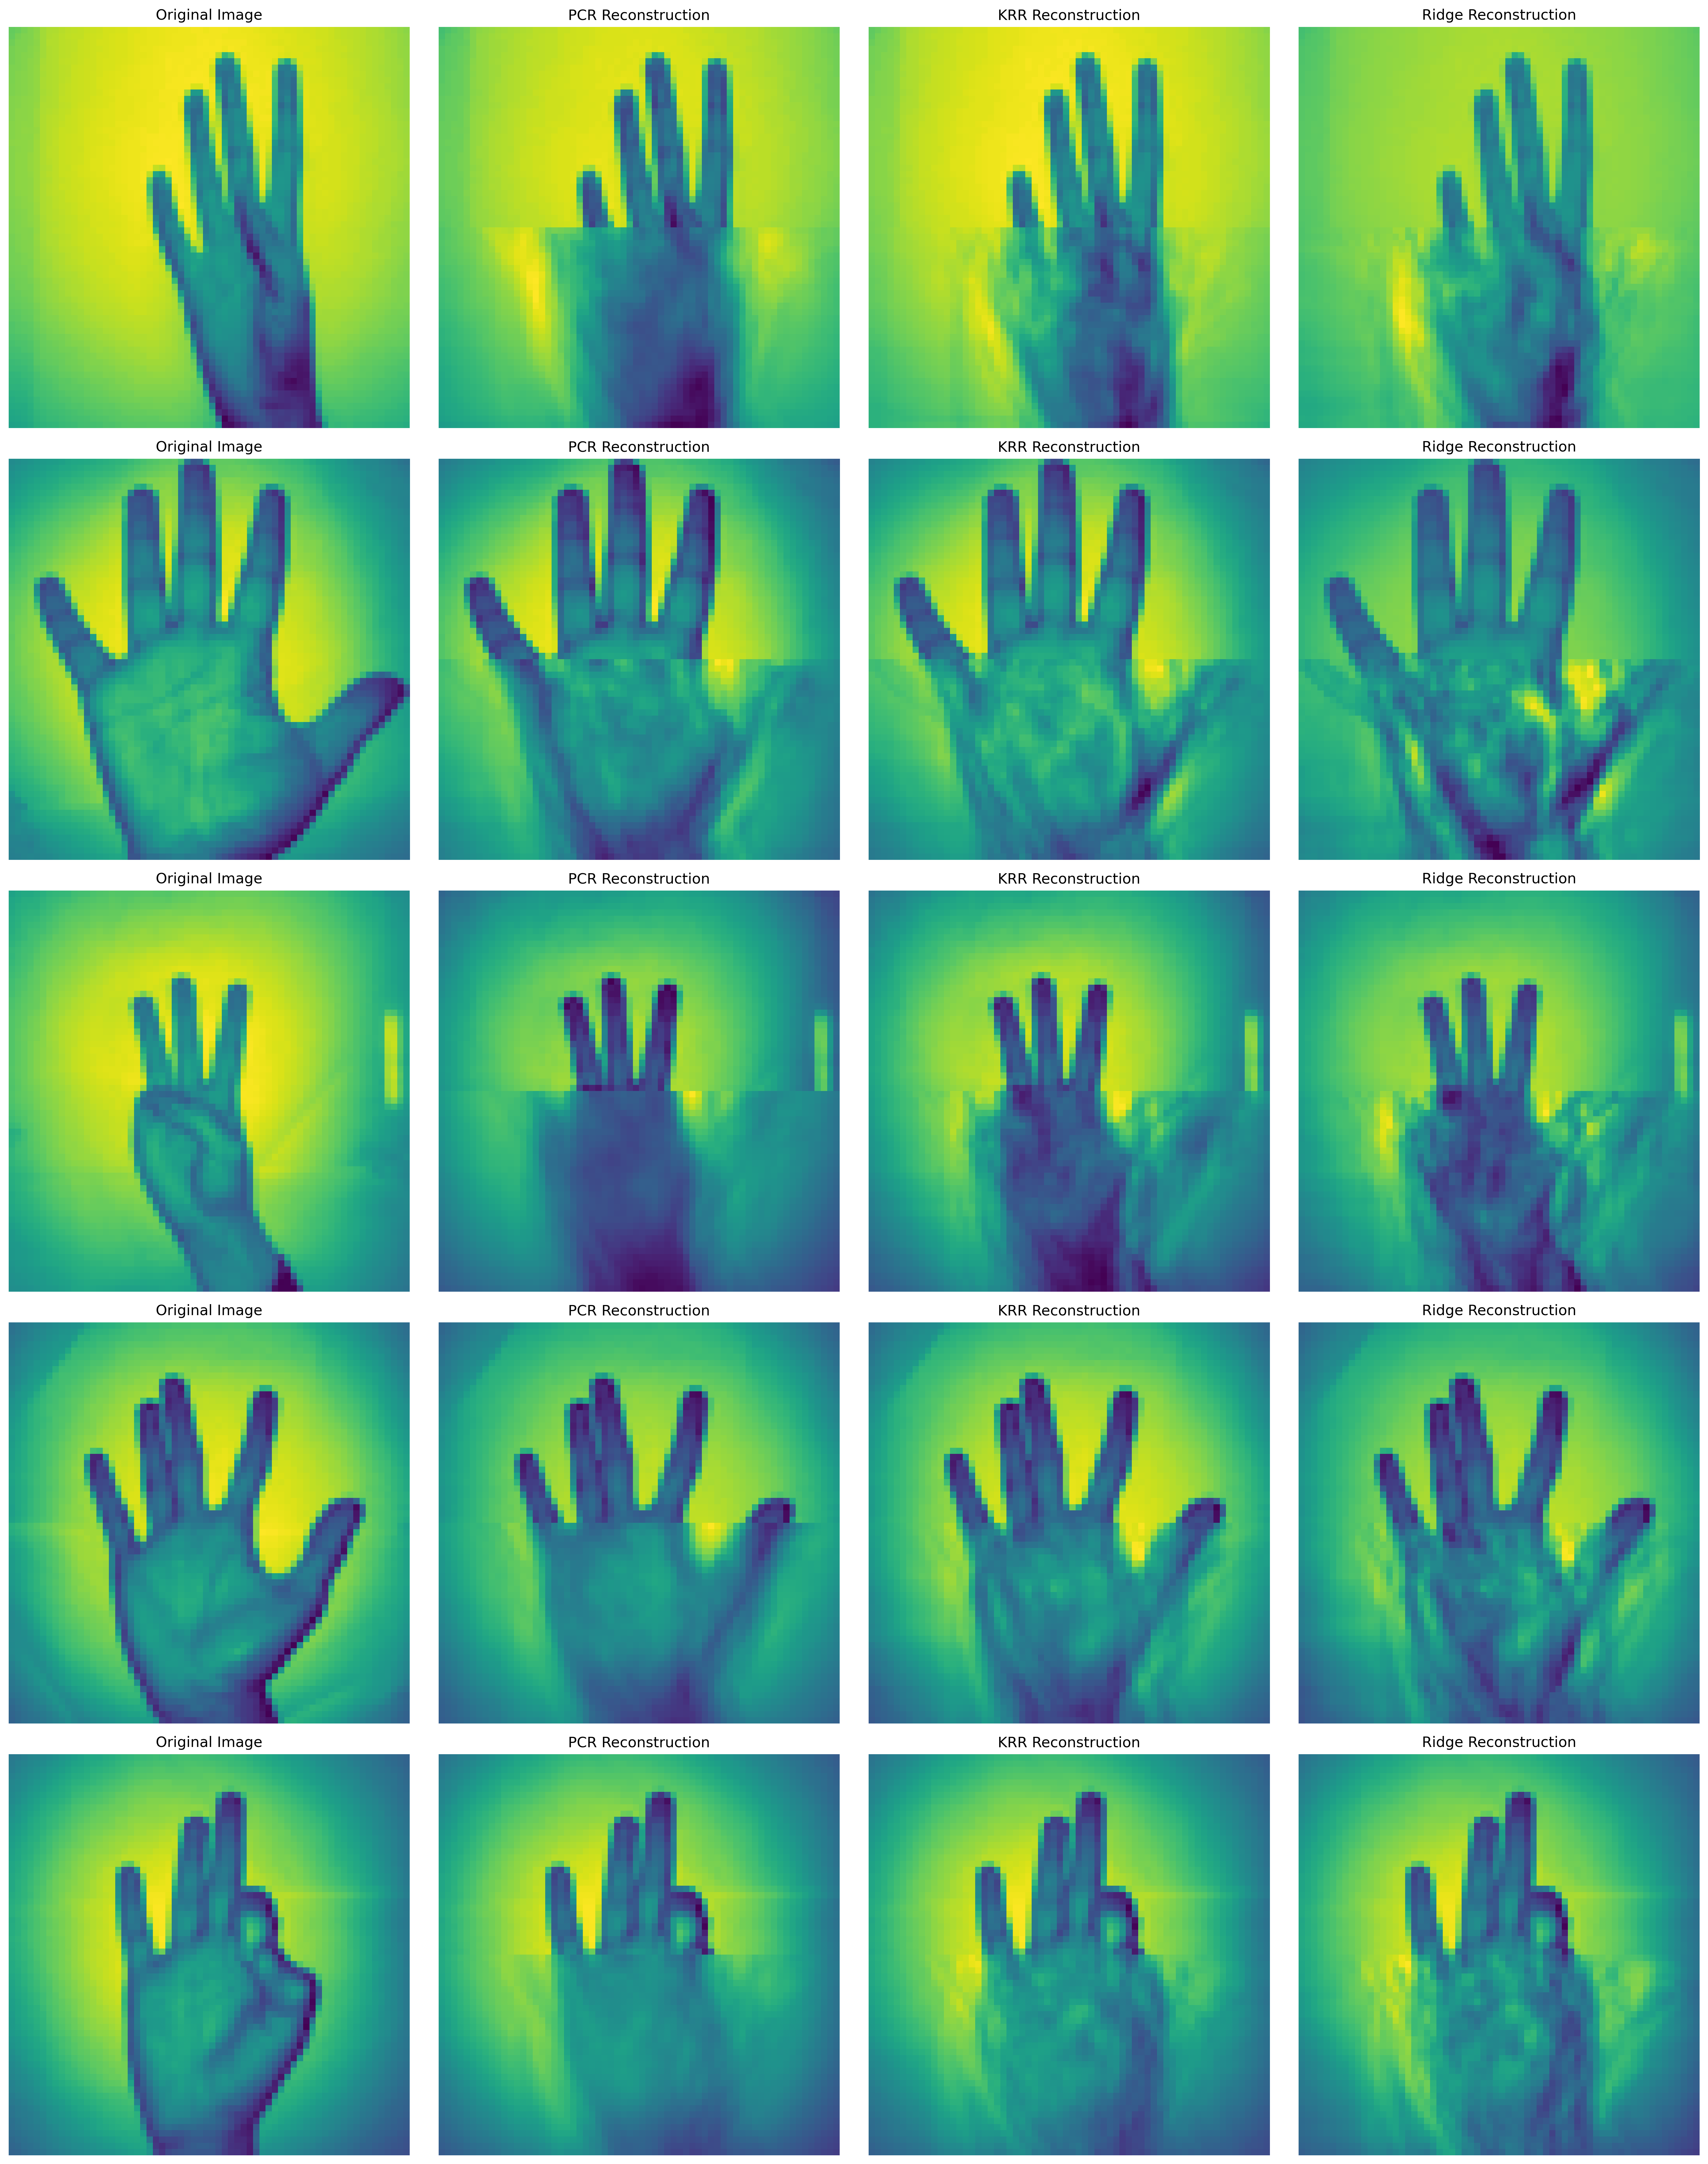
\includegraphics[width=\textwidth]{Task_2/image_completion_comparison.png}
    \caption{Comparison of image completion results using different regression methods. From left to right: Original image, PCR reconstruction, KRR reconstruction, and Ridge reconstruction.}
    \label{fig:completion_comparison}
\end{figure}

\end{appendices}

\end{document}